\subsection*{\textsf{\normalsize 2.2\hspace{0.5cm}KONSEP RANCANGAN}}
\addcontentsline{toc}{subsection}{2.2 KONSEP RANCANGAN}
\hyphenation{di-ba-ngun se-te-ngah}

\begin{figure}
	\centering
		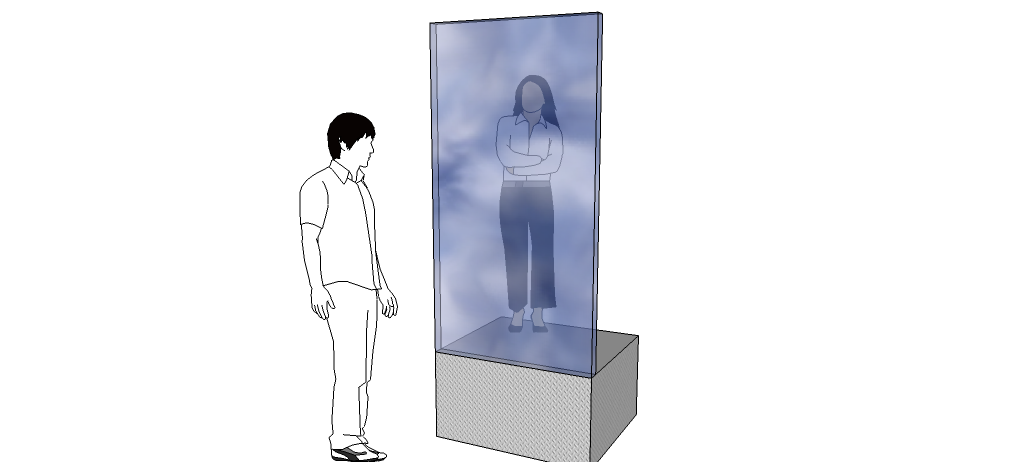
\includegraphics[scale=0.4]{konsep}
	\caption{Konsep instalasi PUSPA}
	\label{fig:konsep}
\end{figure}
Gambar~\ref{fig:konsep} menunjukkan ilustrasi instalasi PUSPA. Pada gambar tersebut terlihat seorang pengguna sedang berinteraksi dengan PUSPA melalui terminal \textit{holoscreen}. Di dalam terminal terlihat seorang asisten yang siap berinteraksi dengan pengguna. Asisten akan melirik ke kiri, kanan, bawah, maupun atas sesuai dengan posisi pengguna. Ia hanya akan diaktifkan jika pengguna adalah benar pemilik PUSPA, yang dapat dipastikan dengan mengenali wajahnya. Interaksi dengan PUSPA layaknya interaksi dengan manusia, yaitu komunikasi \textit{audiovisual}. Dia memiliki kepribadian, ekspresi, penglihatan dan pendengaran. Hal ini membuat seolah-olah PUSPA benar-benar hadir dalam kehidupan nyata. Inilah konsep dasar PUSPA.

PUSPA terdiri dari dua subsistem.
Subsistem pertama adalah subsistem \textit{server}, yang menjadi tempat pengolahan yang berhubungan dengan pembangkitan tanggapan.
Karena konsep PUSPA adalah \textit{client/server},
dimungkinkan agar PUSPA dapat berpindah-pindah terminal sesuai dengan posisi ruangan pengguna.
Subsistem ini menangani pada subsistem \textit{client} mana PUSPA harus ditampilkan.
Subsistem kedua adalah subsistem \textit{client}, yang berinteraksi dengan pengguna,
dan disebut juga sebagai terminal.

Sebagai sebuah \textit{synthespian},
PUSPA menampilkan rupa karakter dan segala pergerakannya.
Pada tahun 1988 Silicon Graphics dan deGraf-Wahrman Inc. bekerjasama dalam pembuatan animasi yang dikontrol oleh manusia.
Mereka merilis ``Mike The Talking Head'' yang menampilkan kepala yang dapat berbicara. \textit{Synthespian} dalam konsep rancangan PUSPA adalah model 3D kepala hingga setengah tubuh.
Adapun fitur \textit{synthespian} mencakup:
  \begin{itemize}
	\item \textit{photorealistic rendering},
	\item animasi emosi,
	\item animasi vokal,
	\item dan animasi panca indera (khususnya penglihatan).
  \end{itemize}
Daniel Thalmann, et al. dalam artikelnya \textit{Autonomous Virtual Actors Based on Virtual Sensors}, menuliskan bahwa \textit{synthespian} dapat memiliki panca indera melalui sensor.

PUSPA dilengkapi dengan antarmuka untuk interaksi selain yang dengan suara.
UI dalam PUSPA mengadopsi konsep \textit{soft control} dengan UI yang di-\textit{render} pada layar dengan desain yang menarik, dinamis, dan \textit{floating}.
Hal ini diperlukan karena \textit{input} pengguna menggunakan sensor sentuh.

Di samping semua itu,
PUSPA juga dilengkapi dengan \textit{multitouch holoscreen},
yang merupakan sebuah layar transparan dengan kemampuan \textit{touchscreen} multi-sentuh.
Contoh penerapan teknologi ini adalah pada produk Microsoft TouchLight.
Gambar~\ref{fig:tlight1} menunjukkan konfigurasi instalasi \textit{holoscreen},
dan Gambar~\ref{fig:tlight2} menggambarkan kemampuan multisentuh TouchLight.
Layar seperti inilah yang akan dikembangkan sebagai terminal PUSPA.
\begin{figure}
	\centering
		\subfloat[\textit{Holoscreen}]{\label{fig:tlight1}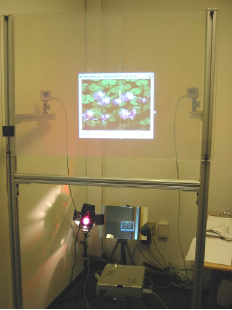
\includegraphics[scale=0.6]{tlight1}}\\
		\subfloat[\textit{Multitouch}]{\label{fig:tlight2}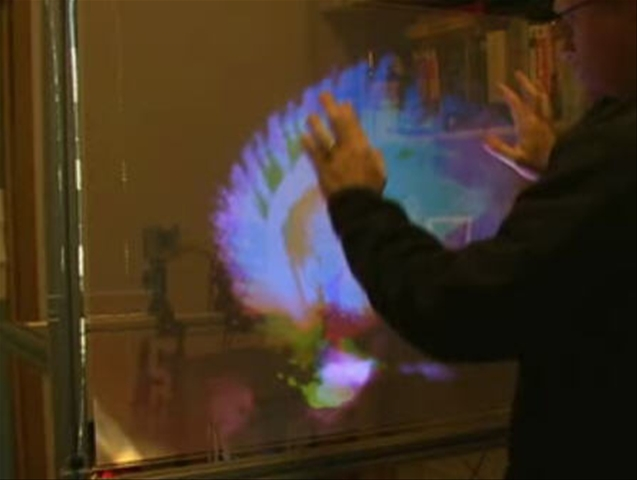
\includegraphics[scale=0.4]{tlight2}}
	\caption{Konfigurasi dan penggunaan touchlight}
	\label{fig:tlight}
\end{figure}	
